\chapter{Sistema de reconocimiento de gestos propuesto}\label{capit:cap3}
\vspace{-2.0325ex}%
\noindent
\rule{\textwidth}{0.5pt}
\vspace{-5.5ex}% 
\newcommand{\pushline}{\Indp}% Indent puede ir o no :p 

En este cap\'itulo se describen las etapas del sistema de reconocimiento de gestos propuesto, junto con los métodos o algoritmos que son utilizados en cada una de ellas.   

El sistema de reconocimiento de gestos propuesto consta de cuatro etapas principales \ref{fig:MyHGR}. La primera etapa es la adquisición de los datos, en la cual se capturan las imágenes de entrada del sistema; la segunda etapa es la detección, aquí la mano es localizada y segmentada del fondo; en la etapa tres se extraen las características de la mano para ser procesadas; en la etapa final el gesto realizado es reconocido.   

\begin{figure}[h!]
\begin{center}
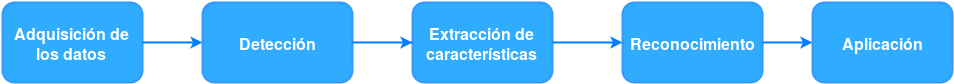
\includegraphics[scale=.6]{./Figures/MyHGR.png}
\end{center}
\caption{Metodología del sistema propuesto.}
\label{fig:MyHGR}
\end{figure}  
  
\section{Adquisición de los datos}\label{sec:KinectSensor} 

Es la primera etapa del sistema, donde se capturan los datos que son la entrada del sistema. Los datos provienen de los sensores de profundidad de dos dispositivos Kinect. A continuación se describe las características de este dispositivo. 

En noviembre del 2010 la compa\'nia Microsoft lanz\'o el sensor Kinect para consolas de vídeo juego Xbox 360 y en febrero del 2011 lanz\'o la versi\'on para Windows, que se muestra en la figura \ref{fig:KinectPic}.  

El dispositivo Kinect esta equipado con una serie de sensores que permiten obtener imágenes a color y de profundidad (imágenes que indican a la distancia que esta un objeto del sensor), los cuales permiten hacer detección y seguimiento de personas. Detecta $6$ personas y hace el seguimiento de $2$ personas \footnote{https://msdn.microsoft.com/en-us/library/hh973074.aspx}.    
  
\begin{figure}[h!]
\begin{center}
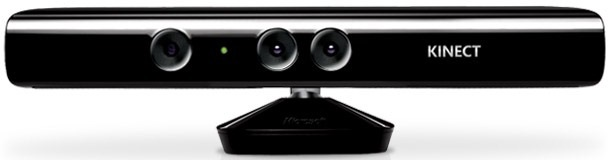
\includegraphics[scale=.60]{./Figures/Kinect.jpg}
\end{center}
\caption{Sensor Kinect para Windows}
\label{fig:KinectPic}
\end{figure} 

El sensor esta equipado con los siguientes componentes: un cámara de color o sensor de color, un emisor infrarrojo, un sensor infrarrojo de profundidad, un motor que controla la inclinación, un arreglo de cuatro micrófonos y un LED \ref{fig:KinectComponentes}. 

Enseguida se describen brevemente cada uno de los componentes del sensor Kinect, \citep{Jana2013}. 
\begin{figure}[h!]
\begin{center}
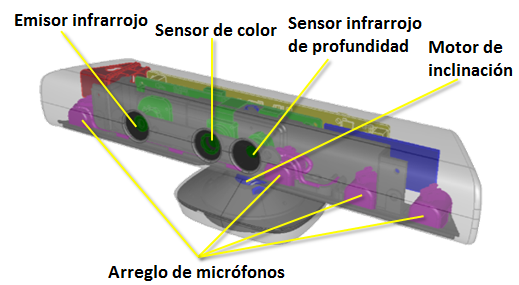
\includegraphics[scale=.6]{./Figures/sensor.png}
\end{center}
\caption{Componentes del sensor Kinect}
\label{fig:KinectComponentes}
\end{figure}   

\begin{itemize}
\item La cámara de color captura y transmite datos de vídeo a color, detectando los colores rojo, verde y azul (RGB, por sus siglas en ingl\'es, red, green and blue). La transmisión de datos que brinda la cámara es una secuencia de imágenes (cuadros), a una velocidad de hasta $30$ cuadros por segundo con una resolución de hasta $1280\, x \, 960$ p\'ixeles. La velocidad de los cuadros por segundo varia según la resolución de la imagen.
\item El emisor infrarrojo proyecta puntos de luz infrarroja frente al sensor, con estos puntos y el sensor de profundidad se puede medir la profundidad que existe del sensor.
\item El sensor infrarrojo lee los puntos infrarrojos proyectados y calcula la distancia que existe entre el objeto y el sensor. El sensor transmite los datos de profundidad con una velocidad de $30$ cuadros por segundo con una resolución de hasta $640 \, x \, 480$ pixeles.   
\item El motor de inclinación controla el \'angulo de la posición vertical de los sensores del dispositivo. El motor puede moverse desde el \'angulo de $-27^ \circ$ a $+27^\circ$. 
\item Arreglo de micrófonos, consta de $4$ micrófonos, captura el sonido y localiza la dirección en la que proviene. 
\item LED indica el estado del sensor.
\end{itemize}



\section{Detección}\label{sec:Detection}

En esta etapa del sistema el objetivo es localizar y segmentar la mano para extraer las características necesarias para el reconocimiento.\\
Este procedimiento se lleve acabo de la siguiente manera, figura  \ref{fig:ProcesoDeteccion} el primer paso es localizar la mano, se lleva acabo usando el método de detección rápida de objetos; el siguiente paso es mejorar la imagen de la mano aplicando operaciones morfológicas y finalmente se la imagen que contiene la mano es binarizada. 

\begin{figure}[h!]
\begin{center}
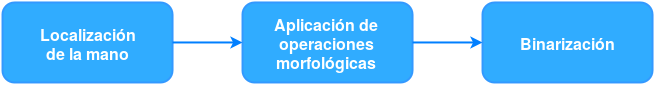
\includegraphics[scale=.7]{./Figures/Detection.png}
\end{center}
\caption{Proceso de detección de la mano.}
\label{fig:ProcesoDeteccion}
\end{figure} 

\subsection{Método detección rápida de objetos usando características simples utilizando el clasificador AdaBoost en forma de cascada}\label{subsec:ViolaJones}

En este trabajo se utiliza el método detección rápida de objetos usando características simples utilizando el clasificador AdaBoost en forma de cascada, \citep{Viola2001}, el cual fue creado originalmente para atacar el problema de detección de rostros, este puede ser usando para detectar cualquier objeto, debido a la forma en que este fue creado, pues detecta un objeto clasificando imágenes basándose en el valor de características simples.

La técnica clasifica si el objeto se encuentra en la escena, usando una versión modificada del clasificador AdaBoost \citep{Freund1995} en forma de cascada, y discrimina el objeto tomando en cuenta el valor de las características Haar \citep{Viola2001}, las características son seleccionadas usando también el clasificador AdaBoost y el valor de estas es calculado mediante el uso de una imagen integral \citep{Viola2001}. 

La figura \ref{fig:ViolaJonesDiagram} muestra un diagrama del proceso del método de detección, el primer paso es obtener la muestras de entrenamiento con las cuales se construirá el clasificador; el siguiente paso es seleccionar las características que formaran el clasificador, estas se escogen mediante el algoritmo de AdaBoost y su valor es calculado usando la imagen integral; el paso final que es construir el clasificador es utilizando 
Adaboost en forma de cascada.

\begin{figure}[h!]
\begin{center}
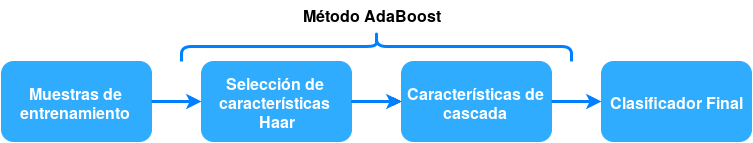
\includegraphics[scale=.6]{./Figures/ViolaJonesDiagram.png}
\end{center}
\caption{Procedimiento del algoritmo de detección}
\label{fig:ViolaJonesDiagram}
\end{figure}

Enseguida se explica a detalle cada etapa del método \citep{Viola2001}. 

\subsubsection{Características Haar}\label{sssec:CaracteristicasHaar}  

Las características Haar, son operadores rectangulares como los que se muestran en la figura \ref{fig:haarFeatures}. A continuación se explicaran los operadores Haar básicos:
\begin{itemize}
\item Las características con dos rectángulos \ref{fig:haarFeatures:1}, \ref{fig:haarFeatures:2}, contienen dos regiones rectangulares adyacentes, y el valor de la característica se calcula tomando la diferencia de la suma de ambas regiones. 

\item Las características con tres rectángulos \ref{fig:haarFeatures:3}, contienen tres regiones rectangulares adyacentes, y el valor de la característica se calcula la suma de las regiones exteriores y se resta la suma de la región interior.

\item Las características con cuatro rectángulos \ref{fig:haarFeatures:4}, contienen cuatro regiones rectangulares adyacentes, y el valor de la característica se obtiene con la diferencia entre las regiones pares diagonales.
\end{itemize} 

\begin{figure}[h!]
\centering
\subfigure[]{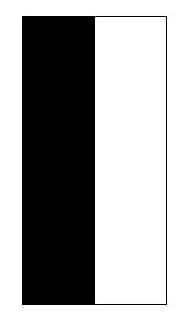
\includegraphics[scale=.4]{./Figures/haarFeatures1}\label{fig:haarFeatures:1}}
\subfigure[]{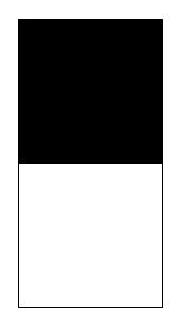
\includegraphics[scale=.4]{./Figures/haarFeatures2}\label{fig:haarFeatures:2}}
\subfigure[]{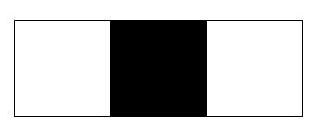
\includegraphics[scale=.4]{./Figures/haarFeatures3}\label{fig:haarFeatures:3}}
\subfigure[]{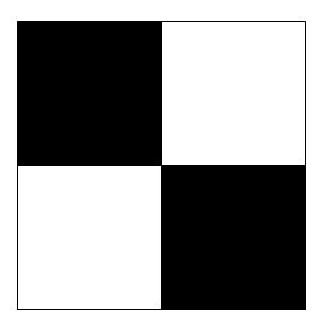
\includegraphics[scale=.4]{./Figures/haarFeatures4}\label{fig:haarFeatures:4}}
\caption{Ejemplo de operadores Haar} \label{fig:haarFeatures}
\end{figure}


\subsubsection{Imagen integral}\label{sssec:IntegralImage} 

Uno de los aportes del método desarrolla por Viola y Jones es el concepto de imagen integral con la cual se calcula el valor de las características de manera rápida, es decir el tiempo constante. 

La imagen integral, $SI$, de un imagen, $S(x,y)$, es calculada como la suma del valor de los pixeles que se encuentran arriba y a la izquierda de cierta posición de la imagen a la cual se quiere hacer el cálculo. Lo anterior se puede escribir como: \footnote{https://computersciencesource.wordpress.com/2010/09/03/computer-vision-the-integral-image/}     
$$SI(x,y)=S(x,y) + S(x-1,y) + SI(x,y-1)-SI(x-1,y-1)$$ 
La figura \ref{fig:FigIntegralImage} muestra un  ejemplo donde se calcula la imagen intregral, fig. \ref{fig:FigIntegralImage:2}, de la imagen original \ref{fig:FigIntegralImage:1}.
\begin{figure}[h!]
\centering
\subfigure[Imagen original]{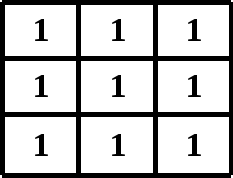
\includegraphics[scale=.7]{./Figures/ImagetoIntegral}\label{fig:FigIntegralImage:1}} \qquad
\subfigure[Imagen integral]{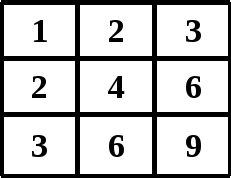
\includegraphics[scale=.7]{./Figures/CalculationIntegral}\label{fig:FigIntegralImage:2}}
\caption{Ejemplo del cálculo de la imagen integral} \label{fig:FigIntegralImage}
\end{figure}

La imagen integral permite calcular la suma de los pixeles de cierta región usando solo los valores de las esquinas de la imagen integral de dicha región, la cual se obtiene como: \footnote{https://computersciencesource.wordpress.com/2010/09/03/computer-vision-the-integral-image/}   
$$REG(\alpha)=SI(A)+SI(D)-SI(B)-SI(C)$$
donde $REG(\alpha)$ es la región a la cual se quiere calcular el valor de la suma de sus pixeles; $A,B,C,D$ son las esquinas de dicha región, como se muestra en la figura \ref{fig:figImageIntegral}, la region $\alpha$ se encuentra resaltada en color azul.  
\begin{figure}[h!]
\begin{center}
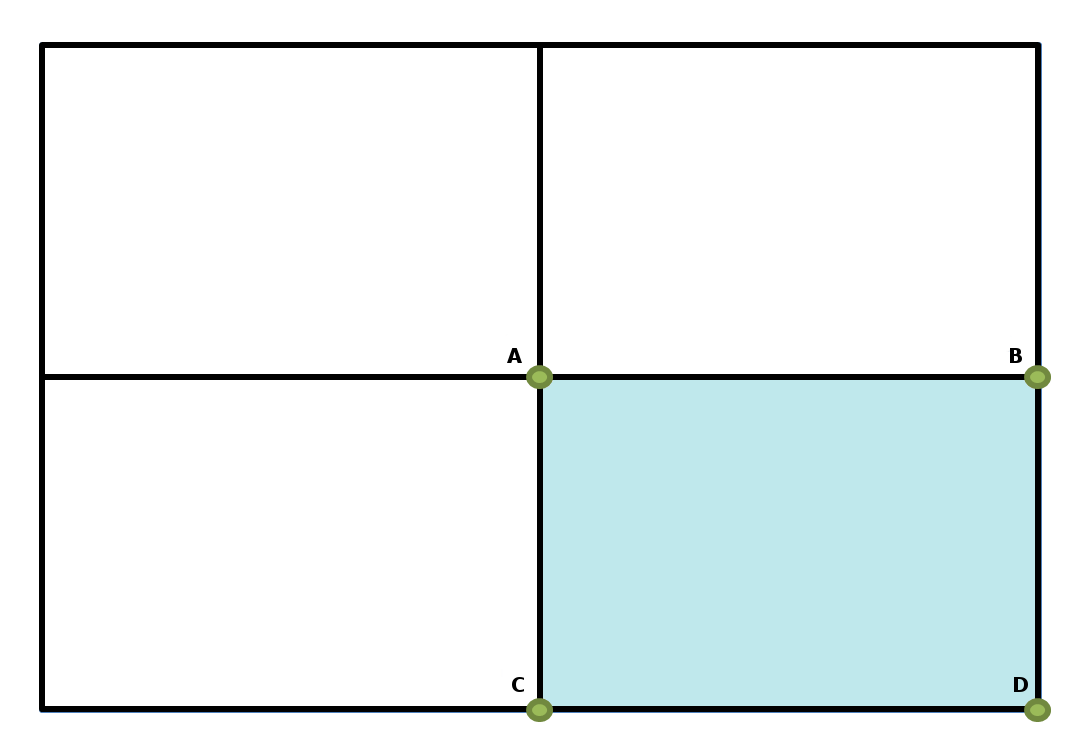
\includegraphics[scale=.3]{./Figures/IntegralImage.png}
\end{center}
\caption{Regiones de la imagen integral}
\label{fig:figImageIntegral}
\end{figure} 


\subsubsection{Algoritmo AdaBoost}\label{sssec:AdaboostClasifier}  

En el método de detección el clasificador AdaBoost es utilizado para seleccionar las características relevantes, con las cuales se podrá detectar el objeto. 

El algoritmo AdaBoost realiza su clasificación construyendo un clasificador fuerte, $h(x)$, llamado así debido a que tiene una precision mayor que los otros clasificadores con los que es construido, clasificadores débiles, $h_i(x)$. Los clasificares débiles son calculados de la siguiente manera: 
$$h_i(x)=
\begin{cases}   
1, \quad Si \quad  p_if_i(x)<p_i \theta_i \\
0, \quad de \quad otra \quad forma.\\
\end{cases}$$
donde $x$ es una sub ventana de la imagen, $f_i(x)$ es una característica, $\theta$ es un umbral, y $p_i(x)$ representa el signo de la desigualdad.   

El clasificador fuerte es una combinación lineal de los clasificadores débiles, y se define de la siguiente forma: 
$$h(x)= \alpha_1h_1(x)+\alpha_2h_2(x)+ \cdots +\alpha_nh_n(x)$$ 
donde $n$ es el n\'umero de características, $\alpha_i$ es el valor asociado a cada característica, el cual va entre $0$ y $1$.


Enseguida se presenta el algoritmo de AdaBoost:

\begin{algorithm}
\begin{algorithmic}[1]

\REQUIRE El conjunto $\lbrace (x_1,y_1), \cdots, (x_n,y_n) \rbrace$ donde $x_i$ representa las imágenes de entrenamiento, $y_i=0,1$ representa las imágenes negativas y positivas respectivamente. 
\ENSURE El clasificador fuerte $h(x)$.  

\STATE Se inicializan los pesos $w_{1,i}=\frac{1}{2m} , \frac{1}{2l}$ para $y_i=0,1$ respectivamente, donde $m$ y $l$ son el número de imágenes negativas y positivas respectivamente.  

\FOR {$t=1$ hasta $T$}   

	\STATE Se normalizan los pesos 
	$$w_{t,i}=\frac{w_{t,i}}{\sum_{j=1}^n w_{t,j}}$$ 
	para que $w_t$ sea una distribución  de probabilidad. 	
	
	\FOR {cada características $j$} 
	Entrenar un clasificador $h_j$ donde se utiliza una sola característica. 
	El error $\epsilon$ es evaluado con respecto a $w_t$, 
	$$\epsilon = \sum_i w_i | h_i(x_i) - y_i |}$$ 
    \ENDFOR
	
	\STATE Escoger el clasificador $h_i$ con el error más pequeño. 
	
	\STATE Se actualizan los pesos  
	$$w_{t+1,i}=w_{t,i} \beta_t^{1-e_i}$$ 
	donde $\beta_t = \frac{\epsilon_T}{1-\epsilon_t}$, 
	$e_i=0$ si $x_i$ es clasificado correctamente de otra forma $e_i=1$. 
	
\ENDFOR  

\STATE El clasificador final o clasificador fuerte es: 
$$ h(x) = 
\begin{cases}  
1, \quad \sum_{t=1}^T \alpha_th_t(x) \geqslant \frac{1}{2}\sum_{t=1}^T \alpha_t. \\  
0, \quad de \quad otra \quad forma. 
\end{cases} $$
donde $\alpha_t = \log{\frac{1}{\beta_t}}$.

\caption{}\label{alg:AdaBoost}
\end{algorithmic}
\end{algorithm} 


\subsubsection{Clasificador AdaBoost en Cascada}\label{sssec:AdaboostCascade}   

El objetivo de realizar la detección utilizando un clasificador en forma de cascada es descartar de manera rápida las regiones donde no se encuentra el objeto. Lo cual se realiza seleccionando las características relevantes que se evalúan primero.  
Esta selección se realiza como lo muestra el algoritmo \ref{alg:Cascade}  cumpliendo cierto valor en la precision  de la detección y del número de falsos positivos. 
El clasificador en cascada \ref{fig:Cascade} esta compuesto por etapas cada una de estas es un clasificador fuerte que es entrenado por medio de AdaBoost. 

\begin{figure}[h!]
\begin{center}
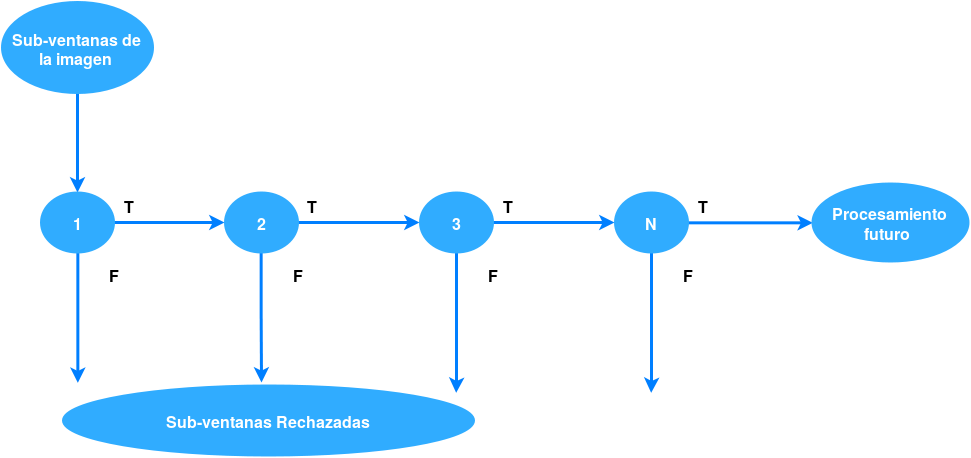
\includegraphics[scale=.5]{./Figures/DCascade.png}
\end{center}
\caption{Clasificador en forma de cascada}
\label{fig:Cascade}
\end{figure} 


\begin{algorithm}
\begin{algorithmic}[1]
\REQUIRE Imágenes positivas $P$, negativas $N$, $f$ el valor máximo de precisión de falsos positivos por etapa, $d$ es el valor mínimo de precisión de la detección por etapa, . 
\ENSURE El clasificador en forma de cascada.  

\STATE  $F_0 = 1$, $D_0=1$

\STATE  $i=0$ 

\WHILE {$F_i > F_{Tarjet}$} 
	\STATE $i=i+1$
	\STATE $n_i=0$, $F_i=F_{i-1}$
	\WHILE {$F_I > F \times fp_{i-1}$} 
		\STATE $n_i = n_i +1$ 
		\STATE Entrenar un clasificador usando AdaBoost con $P$, $N$ y $n_i$ características. 
		\STATE Evaluar el clasificador de cascada para determinar $F_i$ y $D_i$ en el conjunto de validación. 
		\STATE Decrementar el umbral para el $i$-ésimo clasificador hasta que el actual clasificador en cascada tenga un grado 			de detección de por lo menos $d \times D_i-1$.
	\ENDWHILE
	\STATE $N=0$ 
	\IF {$F_i > F_{Tarjet}$} 
		\STATE Evaluar el actual clasificador en cascada en el conjunto de imágenes negativas y poner cualquier detección 				falsa en el conjunto $N$.
	\ENDIF

\ENDWHILE    
\caption{}\label{alg:Cascade} 
\end{algorithmic}
\end{algorithm} 


\subsection{Binarización}\label{subsec:Binarization} 

La binarización es una técnica de procesamiento de imágenes, la cual se encarga de transformar una imagen en escala de grises $S(x,y)$ en una imagen binaria $B(x,y)$ es decir, los pixeles de la imagen toman un valor de $0$ ó $1$.   
Para formar la imagen binaria un valor, umbral, de la imagen en escala de grises es seleccionado. Ya que se tiene el umbral, $T$,     
los pixeles de la imagen son discriminados dependiendo si su valor es mayor o igual al umbral entonces el valor de los pixeles en la imagen binaria es $1$ el resto toma valor de $0$. Es decir: 
$$B(x,y)=
\begin{cases}   
1, \quad Si \quad S(x,y)\geq T \\
0, \quad de \quad otra \quad forma.\\
\end{cases}$$

Existen diversas técnicas para binarizar una imagen, estas se pueden clasificar en dos grupos dependiendo de la manera es que es calcula el umbral, global o local. Los métodos globales calculan un umbral que es usado en toda la imagen y los métodos locales calculan varios umbrales para ciertas regiones de la imagen \citep{Chaki2014}.  

Un método de binarización muy utilizado es el de NiBlack,\citep{Niblack1985} es un método local y adaptativo ya que adapta el umbral basándose en la media $m(i,j)=$ y la desviación estándar $\sigma(i,j)$ de una ventana deslizante de tamaño $bxb$. El umbral $T$  se calcula como: 
$$T(i,j)=m(i,j)+k \cdot \sigma(i,j)$$ 
donde $k \in [0,1]$ el valor de la constante determina que tanta parte del contorno es preservado \citep{Chaki2014}.


  
\subsection{Operaciones Morfológicas}\label{subsec:OperacionesMorfologicas} 

Otra técnica muy utilizada en procesamiento de imágenes son las operaciones morfológicas que son un conjunto de operaciones no lineales, la idea es que al aplicar alguna de estas operaciones el ruido se removido tomando en cuanta la forma y estructura de la imagen. 
La operaciones morfológicas utilizan un elemento estructural el cual se aplica por toda la imagen, los elementos estructurales pueden ser de distintas formas como \ref{fig:EX}

\begin{figure}
\centering
\subfigure[Rectángulo de $3x3$.]{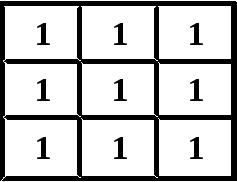
\includegraphics[scale=.7]{./Figures/EX1}\label{fig:EX:1}} %\hspace{20mm}
\qquad
\subfigure[Figura de $3x2$.]{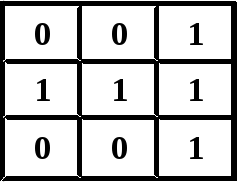
\includegraphics[scale=.7]{./Figures/EX3}\label{fig:EX:3}} 
\\
\subfigure[Cruz de $5x5$.]{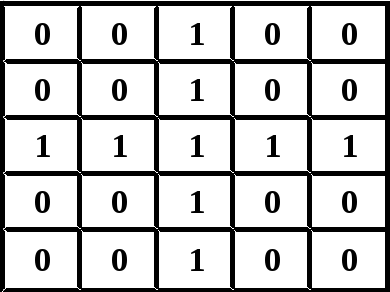
\includegraphics[scale=.7]{./Figures/EX2}\label{fig:EX:2}}
\caption{Ejemplos de elementos estructurales} \label{fig:EX}
\end{figure} 

Existen distintas operaciones morfológicas, las principales o básicas son la dilatación y erosión las cuales se explican enseguida junto con la apertura y cierre. 
 
\subsubsection{Dilatación}\label{sssec:Dilatation}

La dilatación es una operación que añade pixeles a la orilla de los objetos que se encuentran en la imagen. La dilatación se define como:  
$$S \oplus EX = \lbrace S|EX_S \subseteq S \rbrace$$  
donde $EX_S$ es el elemento estructural trasladado con la imagen. 

\subsubsection{Erosión}\label{sssec:OMerosion}

La erosión remueve pixeles a la orilla de los objetos que se encuentran en la imagen. La erosión se define como: 
$$S \ominus EX = \lbrace S|EX_S \subseteq S \rbrace$$ 
donde $EX_S$ es el elemento estructural trasladado con la imagen. 

\subsubsection{Apertura}\label{sssec:Opening} 

La operación apertura abre huecos entre objetos conectados por un enlace delgado de pixeles.  
$$S \circ EX = (S \ominus EX) \oplus EX $$

\subsubsection{Cierre}\label{sssec:Closure}

La operación cierre elimina huecos pequeños  y rellena huecos en las
$$S \bullet EX = (S \oplus EX) \ominus EX $$


\begin{figure}
\centering
\subfigure[original]{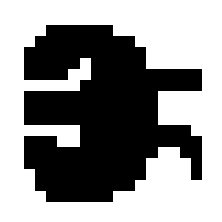
\includegraphics[scale=.7]{./Figures/originalMO}\label{fig:OM:1}} \hspace{10mm}
\subfigure[dilatación]{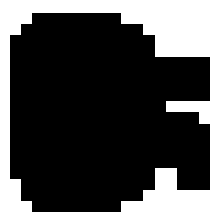
\includegraphics[scale=.7]{./Figures/dilatationMO}\label{fig:OM:2}} \hspace{10mm}
\subfigure[erosión]{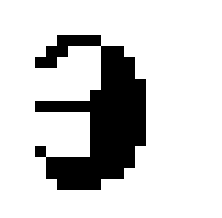
\includegraphics[scale=.7]{./Figures/erosionMO}\label{fig:OM:3}} \hspace{10mm}
\subfigure[apertura]{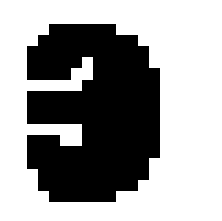
\includegraphics[scale=.7]{./Figures/openingMO}\label{fig:OM:4}} \hspace{10mm}
\subfigure[cierre]{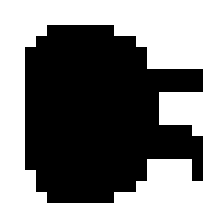
\includegraphics[scale=.7]{./Figures/closingMO}\label{fig:OM:5}}
\caption{Aplicación de operaciones morfológicas (citar)} \label{fig:OM}
\end{figure} 



\section{Extracción de características}\label{sec:Convexhull} 

La idea de esta etapa es obtener las características de la imagen que sean capaces de describir la mano, de manera que con estas, se pueda reconocer los gestos realizados.\\     
En este trabajo se extraen características geométricas, las cuales son extraídas de la siguiente forma: el primer paso es encontrar la envolvente convexa de la mano para posteriormente calcular los defectos de convexidad una vez realizado lo anterior se pueden calcular el numero de dedos de la mano entre otras características; finalmente las características calculadas  se guardan en un vector.  

\begin{figure}[h!]
\begin{center}
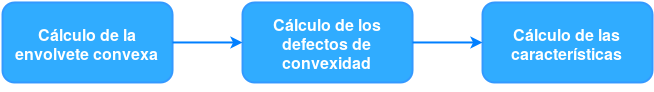
\includegraphics[scale=.7]{./Figures/DExtraccion.png}
\end{center}
\caption{Proceso de la extracción de características.}
\label{fig:DiagramaExtraccionCaracteristicas}
\end{figure} 

A continuación se definen los conceptos anteriores y el de conjunto convexo.

Sea $A$ un conjunto en el espacio euclidiano $\bold{R}^d$, $A$ es un conjunto convexo \footnote{Weisstein, Eric W. "Convex." From MathWorld--A Wolfram Web Resource. http://mathworld.wolfram.com/Convex.html} si contiene todos los segmentos de línea que unen a cualquier par de puntos pertenecientes al conjunto. Donde $d$ es la dimensión del espacio euclidiano. 
\begin{figure}[h!]
\centering
\subfigure[Conexo]{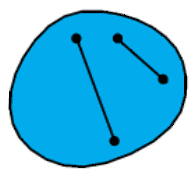
\includegraphics[scale=.8]{./Figures/ConvexSet.png}\label{fig:Sets:Convex}} \hspace{10mm}
\subfigure[convexo]{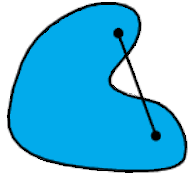
\includegraphics[scale=.75]{./Figures/ConcaveSet.png}\label{fig:OM:Concave}} \hspace{10mm}
\caption{Conjunto conexo y convexo (citar)}\label{fig:Sets}
\end{figure} 

Sea $B$ un conjunto de puntos en el plano Euclidiano, la envolvente convexa de $B$ es el conjunto convexo más pequeño que contiene a todos los puntos en $B$. En la imagen \ref{fig:FigConvexHullDefects} se muestra de color rojo la envolvente convexa de la figura cuyo contorno se encuentra de color negro. 

Los defectos de convexidad de la envolvente convexa, son el conjunto de puntos que no pertenecen al casco convexo. El defecto es el espacio que existe entre el contorno de la envolvente convexa y del objeto.\\
Sea $CD=\lbrace cd_1, cd_2, \cdots, cd_n \rbrace$ el conjunto de defectos de convexidad de una envolvente convexa. Cada defecto esta compuesto por tres elementos: el punto de inicio del defecto $s_i(x,y)$; el punto con mayor distancia de la envolvente al objeto, $d_i(x,y)$ y el punto final del defecto, $e_i(x,y)$.
En la imagen \ref{fig:FigConvexHullDefects} los puntos amarillos representan los puntos de profundidad de los defectos de convexidad. 

\begin{figure}[h!]
\begin{center}
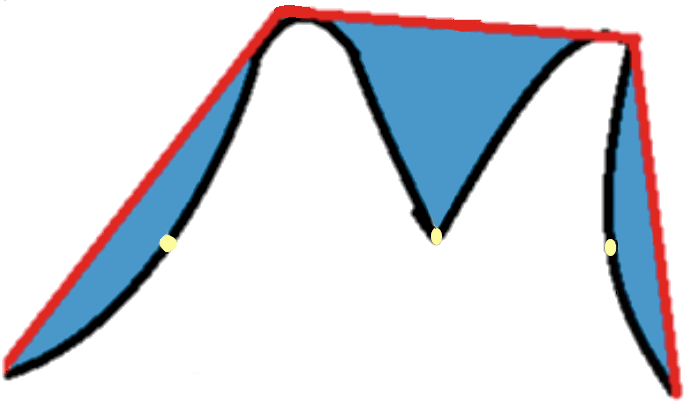
\includegraphics[scale=.4]{./Figures/ConvexHullAndDefects.png}
\end{center}
\caption{En la imagen se aprecia de color rojo la envolvente convexa, de negro el contorno de la figura, y los puntos amarillos son el punto de profundidad de los defectos de convexidad.}
\label{fig:FigConvexHullDefects}
\end{figure}  

Usando las técnicas anteriores podemos extraer características importantes como el numero de dedos, la posición del centro de la mano, el ángulo que existe entre cada dedo. 

El número de dedos que se encuentran levantados es calculado con el algoritmo \ref{alg:NumDedos}, \textbf{referenciar}, que utiliza los defectos de convexidad en especifico los conjuntos de puntos de inicio, $\mathcal{S}=\lbrace s_1(x,y), s_2(x,y), \cdots, s_n(x,y) \rbrace$ y el de mayor distancia, $\mathcal{D}=\lbrace d_1(x,y), d_2(x,y), \cdots, d_n(x,y) \rbrace$, donde $n$ es el número total de defectos de la envolvente convexa.  

\begin{algorithm}[h!]
\begin{algorithmic}[1]
\REQUIRE Los conjuntos $\mathcal{S}$, $\mathcal{D}$.   
\ENSURE Número de dedos, $Nf$.  

\FOR{$i=1$ hasta $n$}  
	\STATE $minDist=20$, $maxAng=60$, $antecesor=0$, $sucesor=0$. 	
	
	\IF{$d_i(x,y) < minDepth$ } 
	\STATE \textbf{continuar} 
	\ENDIF 
	
	\IF{i=0} 
	\STATE $antecesor=n-1$
	\ELSE
	\STATE $antecesor=i-1$
	\ENDIF 

	\IF{i=n-1} 
	\STATE $sucesor=0$
	\ELSE
	\STATE $sucesor=i+1$
	\ENDIF   
	
	\STATE Calcular el ángulo entre $s_{antecesor}(x,y)$, $d_i}$  $s_{sucesor}(x,y)$
	
	\IF{$ \text{ángulo} \geqslant maxAng$}
	\STATE \textbf{continuar}
	\ENDIF  
	
	\STATE $Nf=Nf+1$.
\ENDFOR 

\caption{Calcula el número de dedos de la mano.}
\label{alg:NumDedos} 
\end{algorithmic}
\end{algorithm} 

El ángulo $\alpha$ entre los dedos $Nf_j$ y $Nf_{j+1}$ es calculado como:  
$$ \alpha_{f_j} = \tan^{-1}{ \bigg| \frac{m_{j+1}-m_j}{1+m_{j+1}m_j} \bigg|}$$
donde $m_{j+1},m_j$ son las pendientes de las rectas que pasa por los puntos $d_j(x,y)$ y $s_{j+1}(x,y)$; $d_j(x,y)$ y $s_j(x,y)$; $j=\lbrace 1,2,3,4,5 \rbrace$.  

El ángulo del centro de la mano a la punta de los dedos puede ser obtenido como: 
$$ \theta_{Nf_j} = \tan^{-1} | {m_j} - 90^\circ |$$
donde $m_j$ es la pendiente de la recta que pasa por el centro de la mano y la punta de los dedos $s_i(x,y)$.

Una vez que todas las características son calculas están se guardan en un vector, llamado vector de características. La dimension del vector es el numero de características que este contiene. 


\section{Reconocimiento}\label{sec:SVM} 

Es la etapa final del reconocimiento, es donde finalmente el gesto puede ser interpretado por la computadora.  

En este trabajo el reconocimiento se realiza con el método de máquinas de soporte vectorial (SVM, por sus siglas en ingles, support vector machine), un método de aprendizaje de máquina supervisado que es utilizado para resolver problemas de clasificación y regresión. El cual tiene como objetivo crear un modelo basado en datos conocimos (datos de entrenamiento), que predice a que clase pertenecen datos nuevos. 

SVM realiza la clasificación separando las clases buscando el hiperplano que tengan el margen  de separación más grande. Enseguida se explica a detalle el funcionamiento del método. 

Dado $N$ puntos de entrenamiento $x_i$, de dimensión $D$, dos clases distintas $y_i=-1$
o $+1$ es decir: 
$$\lbrace x_i,y_i \rbrace \quad \text{donde} \quad  i=1, \cdots ,N \quad y\in{-1,1} \quad x \in \Re^D$$  
Hiperplano óptimo  
$$ w \cdot x + b = 0$$ 
donde $w$ es la normal al hiperplano, $\frac{b}{|w|}$ es la distancia perpendicular desde el hiperplano al origen.   
$$ w \cdot x + b = +1 \textrm{ para } y_i=+1$$ 
$$ w \cdot x + b = -1 \textrm{ para } y_i=-1$$ 
Maximizar el margen, encontrar el mínimo de $w$.  
$$Min\Vert w \Vert \quad \text{tal que} \quad y_i(w \cdot x_i + b) -1 \geq 0$$
\begin{figure}[h!]
\begin{center}
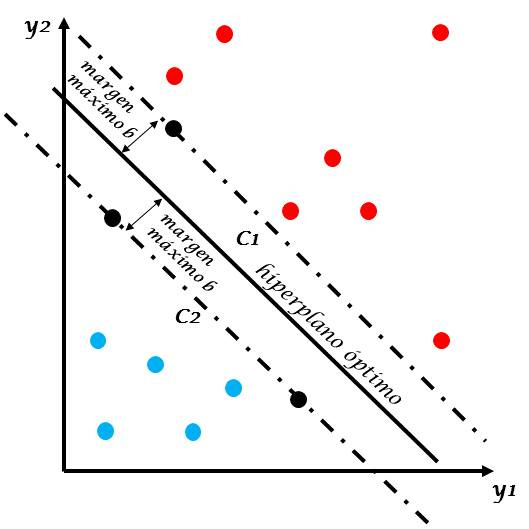
\includegraphics[scale=.3]{./Figures/maquinaSoporte.jpg}
\end{center}
\caption{Clasificación de maquina de soporte usando kernel lineal}
\label{fig:SVM}
\end{figure} 


\newpage
%%=====================================================
